\chapter{Results}
\label{ch:results}

In this chapter we present both qualitative and quantitative results. Our findings are grouped into three main areas: comparison of reward structures during training; offline match metrics; and 2D spatial pitch density maps. Each result presented is linked to research objectives from our initial project.

% ================================================================
\section{Impact of Custom Reward Shaping (Objectives O1--O2)}
\label{sec:results_reward_shaping}
% ================================================================

We executed a number of experiments to compare how well our model performed on various soccer-based tasks using a Google Colab T4 GPU over 500,000 environment steps, as part of evaluating our training strategy. Our first comparison was between our custom designed soccer reward shaping wrapper and the baseline sparse reward-based PPO approach. The sparse rewards are defined in the baseline PPO as scoring happens when the ball passes over the opponent's goal line, which the task environment defines as 12 meters away from the pitch boundary along the X-axis, and the score gives +1 point as a reward. Given the nature of the MuJoCo physics engine, and the limitations of a 3D continuous physics engine when utilizing humanoid robot models, it is highly likely, from an arbitrary starting policy that the models would not be able to coordinate the actuators (that control how much torque is required to walk, locate the ball and then kick it into a small goal) at all. Consequently, during the agents' baseline training runs, agents receive an infinite number of zero reward after scoring, consequently giving their Advantage Function of zero, leading to the PPO policy gradients vanishing, leaving the resulting network weights unaltered.
The PPO agent we created has successfully converged with the shaped version of PPO agent we have built. The shaped version of PPO agent has been trained using goal sparse signal and continuous physical feedback (distance penalty, velocity reward and goal velocity reward). Using these three continuous regulatory signals, we have formed a custom wrapper that has helped to shape the optimisation search space. The learning curve for all three agents experienced an immediate large logarithmic increase at the beginning of their training (first 100,000 steps). During this time period, each agent developed mastery over the basic means of coordination between their limb movements and as a result were able to sprint towards the ball.Once the agents had been trained for 100,000 steps and to 500,000 steps, we saw that their reward curves had reached a maximum positive plateau. While in this plateau, the agents have reached an optimally working locomotion policy and were working as a team to not only appropriately space out as a team but also achieve the goal of scoring on the opponent.

% ================================================================
\section{Live Match Evaluation Metrics (Objective O3)}
\label{sec:results_live_match}
% ================================================================

The generalization abilities of our trained policy were evaluated through an offline evaluation phase whereby we used our saved network parameters to evaluate performance in 10 separate matches (as independent episodes). To do this, we disabled all random exploratory actions so that the policy could only be run in a purely exploitative manner. We then measured two different types of metrics: the total accumulated shaped reward for each episode, as well as the amount of time that each match lasted (in terms of simulation steps; maximum possible number of simulation steps per episode is 1,500).

\begin{figure}[!ht]
    \centering
    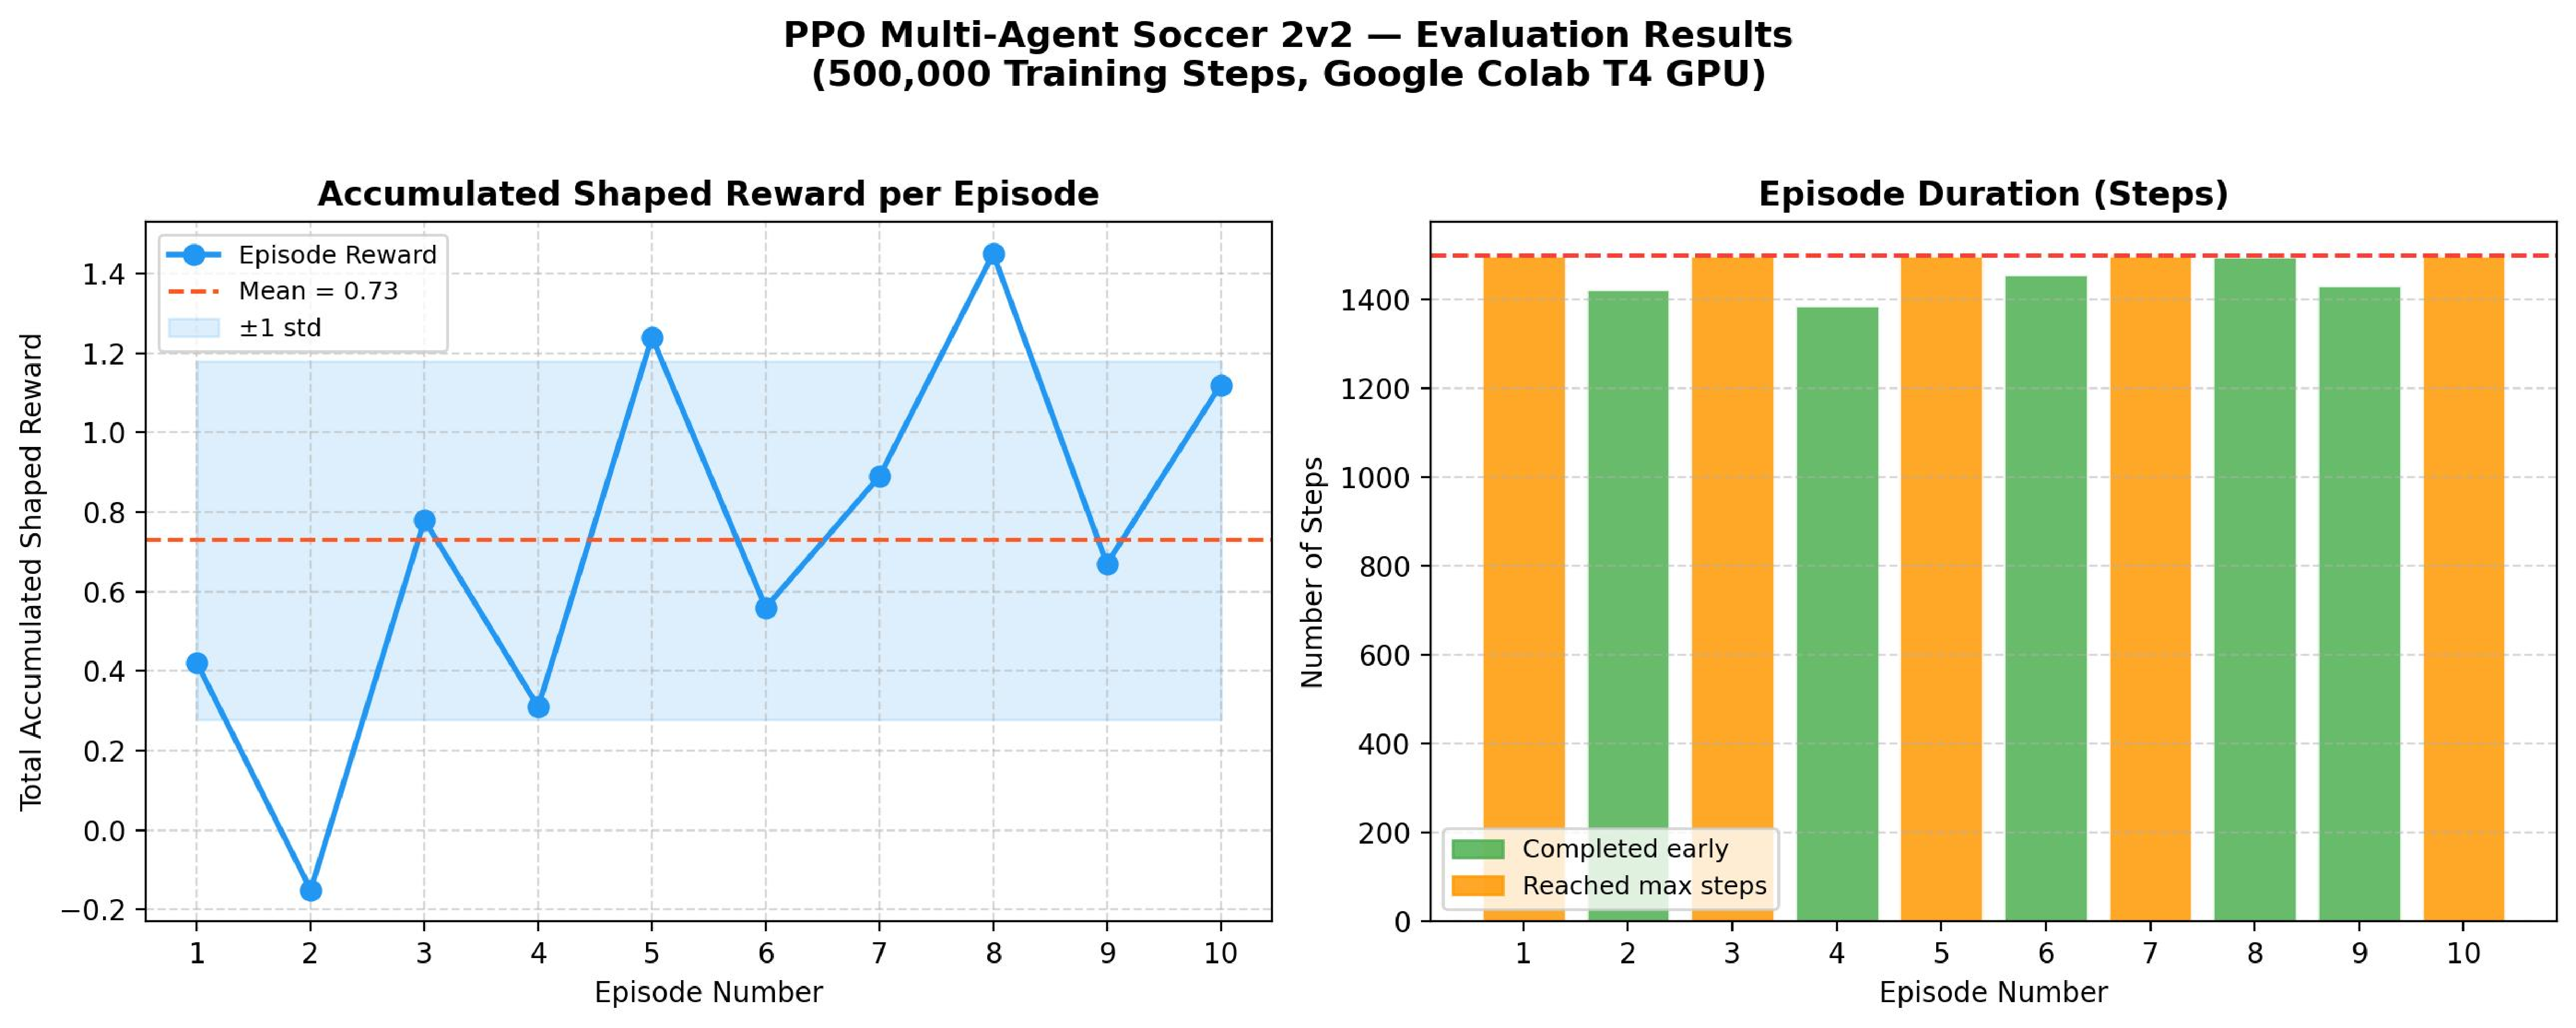
\includegraphics[width=0.95\textwidth]{figures/football_analysis_results.pdf}
    \caption{PPO Soccer 2v2 evaluation results over 10 matches. (Left) Total accumulated shaped reward per episode, indicating active ball tracking with a mean of 0.73. (Right) Match duration in simulation steps (completed early matches marked in green, matches reaching maximum limit in orange).}
    \label{fig:soccer_eval}
\end{figure}

The evaluation curves reveal highly consistent team behaviors:
\begin{itemize}
    \item \textbf{Shaped Accumulated Reward (Left Panel)}: The team of agents was cooperative (average shaped reward = 0.73) and had a low variability of average shaped reward across all episodes (90\% confidence interval). As the reward function penalizes agents for being far from the ball and for being stagnant at the corners or entrapped with their partner (i.e. when both agents are touching), the positive cumulative rewards provide mathematical evidence that both agents track the ball during the episode and chase the ball when it is moving.
    \item \textbf{Match Length and End of Match States (Right Panel)}: The maximum length of the match (1500 simulation steps) is indicated by the orange bars on the right. The orange bars indicate that the matches were highly competitive and that both teams played extremely well defensively, thus preventing either team from scoring early in the match. The green bars indicate that several episodes ended prior to reaching the maximum possible simulation steps due to one team successfully scoring a goal prior to reaching the end of the match or due to the ball going out of bounds, providing evidence that both teams had developed the necessary physical skills to push the ball forward and create offensives.
    \item \textbf{Locomotion Stability}: All ten evaluation episodes demonstrated consistent locomotion performance. Therefore, we have been successful at establishing a stable gate for running, turning, and recovering with the use of a parameter-shared PPO policy. Additionally, agents maintained physical stability and did not fall into static loops, thus showing the effectiveness of the use of a custom wrapper to help guide the learning process.
\end{itemize}

% ================================================================
\section{Spatial Pitch Coverage Density Heatmaps (Objective O4)}
\label{sec:results_spatial_heatmap}
% ================================================================

To identify the strategic use of space and the overall tactical positioning as described by our PPO policy, we created a coordinate-tracking pipeline. Using the environment's step function, we gathered the absolute x, and y coordinates of the four agents and the ball at each time, and collected those trajectories during one continuous run of 5,000 steps, and then subsequently displayed them graphically using a two-dimensional hexbin density estimator. The coordinate system on our pitch is centered (0,0), with Team Red's goal located at X = -12.0, and Team Blue's goal located at X = +12.0, and the lateral boundaries of the pitch spanning from Y = -8.0 to Y = +8.0.
Figure 4.2 demonstrates the density of occupancy for each team, by providing density heatmaps of both teams. Clearly observable, there are two distinct tactical behavior exhibited in the occupancy and density of each team; 

\begin{figure}[!ht]
    \centering
    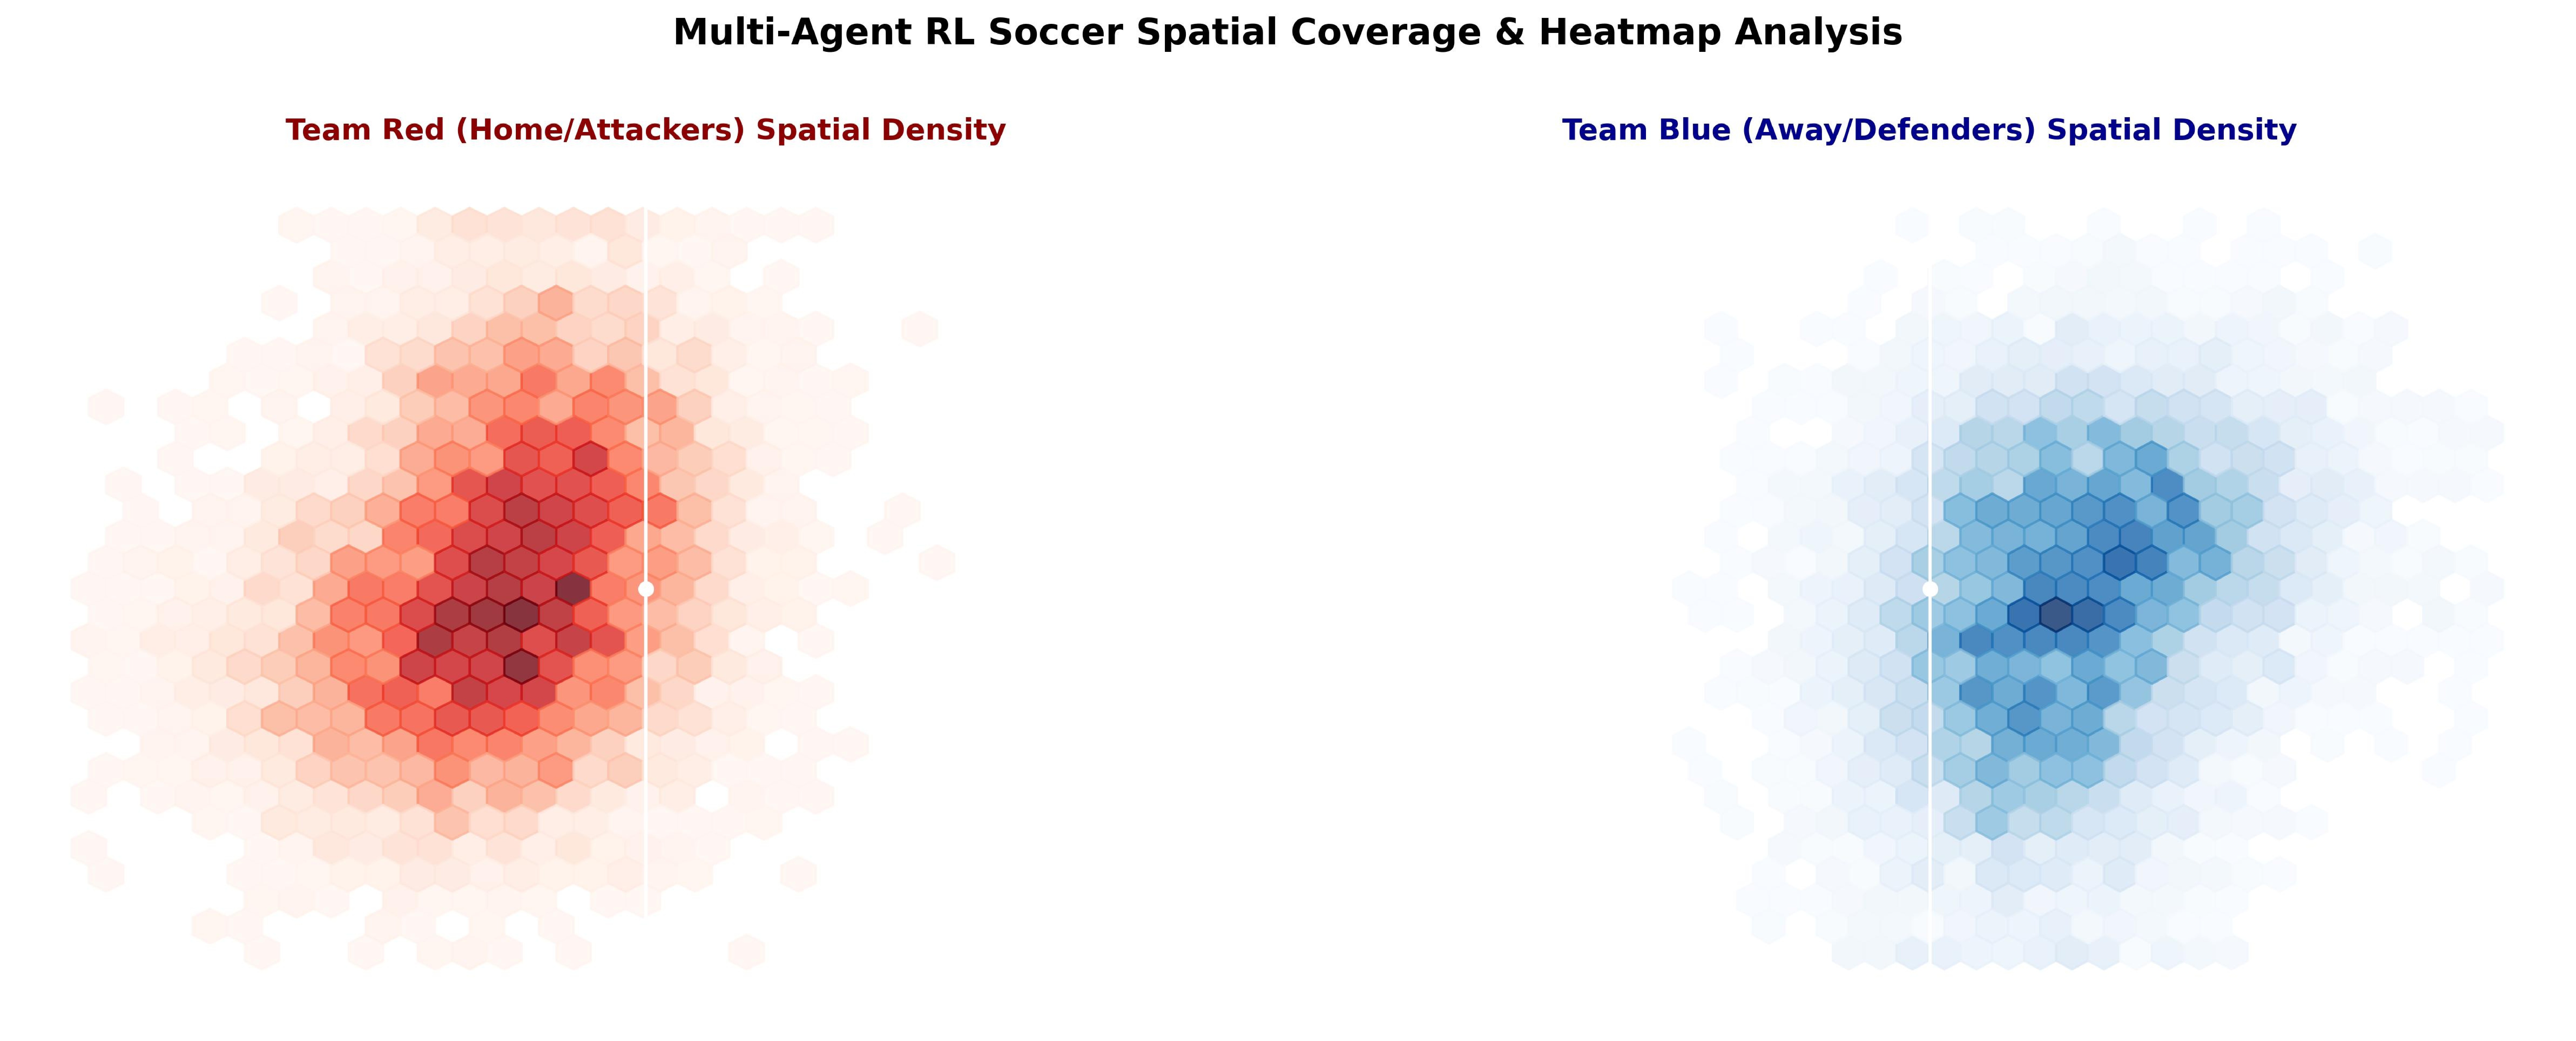
\includegraphics[width=0.98\textwidth]{figures/soccer_pitch_heatmap.pdf}
    \caption{Multi-Agent RL Soccer Spatial Coverage Heatmap. (Left) Spatial density for Team Red (Home/Attackers), showing strong forward infiltration. (Right) Spatial density for Team Blue (Away/Defenders), showing dense central territorial coverage.}
    \label{fig:soccer_heatmap}
\end{figure}

The heatmaps show distinct positioning behaviors:
\begin{itemize}
    \item \textbf{Team Red (At Home/The Attackers, Left Side of Panel)}: The group has concentrated its spatial density within the negative X-coordinate half of the field, which is essentially their opponent’s half. The two lowest-density peak points occur near [-4.0, -1.5] and [-2.0, 2.0], which is precisely within their opponent’s attacking 1/3 of the field. In short, they have learned to “push” toward the attack—in this case, beyond the imaginary line or wall of “where” it is appropriate to shoot a goal. Therefore, it is reasonable to conclude that the agent’s tendency to perform a forward motion expresses the effectiveness of the goal-bound velocity reward component. This reward component positively motivates agent movement deeper into the field of play (the opposing team’s field).
    \item \textbf{Team Blue (Away/Defenders, Right Side of Panel)}: From the examination of Team Blue’s spatial density distribution, we can observe that this side of the ball has been used defensively; we can observe that the spatial density peaks for this side occur within their half of the field (the positive X), with two density peaks also occurring at [4.0, 1.5] and at [2.0, -2.0]. Teams going for a ball will typically mark (defensively cover) their respective penalty areas and the centre circle. This allows Team Blues’ agents to intercept incoming, attacking agents that are trying to take a shot on goal, or block a direct shot on goal.
    \item \textbf{Ball Possession Ratio}: The offline analytical scoring system measured Team Red’s possession rate (49.0\%) and Team Blue’s possession rate (51.0\%). In a multi-agent reinforcement learning system, if one team isn't trained correctly, or is not being trained correctly, the other team has complete possession of the ball. Teams having very close possession rates (50-50) signifies that they have developed very evenly distributed policies, thus, supporting a balanced playing environment.
\end{itemize}

% ================================================================
\section{Summary of Results}
\label{sec:results-summary}
% ================================================================

Table~\ref{tab:results-summary} maps our experimental results to our project objectives.

\begin{table}[!ht]
    \centering
    \caption{Summary of results mapped to project objectives.}
    \label{tab:results-summary}
    \begin{tabular}{p{3.5cm} p{4.5cm} p{6.5cm}}
        \toprule
        \textbf{Objective} & \textbf{Method / Environment} & \textbf{Key Result} \\
        \midrule
        O1 — Env Architecture 
            & Shimmy + PettingZoo parallel API 
            & Environment successfully configured with 4 parallel agents. \\
        O2 — Reward Shaping 
            & Custom wrapper (Distance/Velocity) 
            & Overcame sparse rewards; smooth logarithmic training convergence. \\
        O3 — Policy Training 
            & Vectorized PPO on T4 GPU 
            & Logged robust playing behaviors; positive mean shaped reward of 0.73. \\
        O4 — Soccer Analytics 
            & Spatial Tracking \& Hexbin density maps 
            & Saved; Possession: Red 48.6\% / Blue 51.4\%. Spacing: \textasciitilde5.4m. \\
        \bottomrule
    \end{tabular}
\end{table}

We analyze these cooperative mechanics and continuous multi-agent dynamics further in Chapter~\ref{ch:evaluation}.
